\chapter{Aplikacje WWW}

Materiały teoretyczne zostały opracowane na podstawie materiałów Łukasza Sznuka -- \href{https://moodle.mimuw.edu.pl/course/view.php?id=1375}{kurs na Moodle}.

\section*{Podstawa programowa}
\begin{enumerate}
    \item Rodzina \textbf{protokołów HTTP}.
    \item Mechanizmy tworzenia stron internetowych: \textbf{HTML, CSS}.
    \item Język \textbf{JavaScript} oraz jego unikalne cechy. Języki kompilowane na JavaScript.
    \item \textbf{Mechanizmy budowania aplikacji internetowych}: ciasteczka, żądania, routing, widoki, mapowanie obiektowo-relacyjne.
    \item \textbf{Bezpieczeństwo aplikacji webowych}.
\end{enumerate}

% Julia
\section{HTML i CSS}

\textbf{HTML} to język opisu strony, a \textbf{CSS} to język opisu jej wyglądu.

\subsection{HTML}

Dokument HTML składa się ze \textbf{znaczników} (inaczej nazywanych tagami lub elementami HTML) i można go podzielić na dwie główne części: \textbf{nagłówek} (\textit{head}), który zawiera metadane dokumentu (można w nim używać ograniczonego zestawu znaczników) oraz \textbf{treść strony} (\textit{body}).

\begin{example}
    Poniżej przedstawiono podstawowy szkielet prostej strony internetowej:
    \begin{html}
        <!DOCTYPE html>
        <html>
            <head>
                <!-- Treść nagłówka -->
                <title>Tytuł</title>
            </head>
            <body>
                <!-- Znacznik otwierający - div -->
                <!-- Atrybuty - lang, class, id -->
                <!-- Wartości atrybutów - en, c1 c2, adiv -->
                <div lang="en" class='c1 c2' id=adiv>
                    Treść.
                <!-- Znacznik zamykający - div -->
                </div>
        
                <!-- Znacznik otwierający bez znacznika zamykającego -->
                <img src="https://bit.ly/3vz8t3y">
            </body>
        </html>
    \end{html}
\end{example}

Nagłówek może zawierać między innymi:
\begin{html}
<!-- Tytuł -->
<title>Tytuł</title>

<!-- System kodowania -->
<meta charset="utf8">

<!-- Bazowy URL -->
<base href="https://mimuw.edu.pl/" target="_blank">

<!-- Zewnętrzne linki -->
<link rel="stylesheet" href="style.css">

<!-- Link do skryptu lub jego kod -->
<script src="kod.js"></script>
<script> console.log("!"); </script>

<!-- Kod CSS dotyczący stylu -->
<style> a {color: green;} </style>
\end{html}

Treść strony zawiera między innymi znaczniki, które na stronie wyświetlają się zwykle jako prostokątne pudełka zawierające coś wewnątrz siebie. Tymi znacznikami są:
\begin{itemize}
    \item \htmlinline{<body>} -- cała treść strony
    \item \htmlinline{<header>} -- przeważnie jakaś wstępna treść lub linki, znajduje się na górze strony
    \item \htmlinline{<footer>} -- stopka znajdująca się na dole strony
    \item \htmlinline{<main>} -- główna treść
    \item \htmlinline{<nav>} -- linki nawigacyjne
    \item \htmlinline{<article>} -- niezależna treść
    \item \htmlinline{<aside>} -- treść znajdująca się przeważnie po boku strony, oprócz głównej treści
    \item \htmlinline{<section>} -- sekcja dokumentu
    \item \htmlinline{<div>} -- używany, gdy żaden z powyższych nie pasuje do znajdującej się w znaczniku treści
\end{itemize}

Oprócz tego, w treści strony używane są takie znaczniki jak:
\begin{itemize}
    \item nagłówki: \htmlinline{<h1>}, \htmlinline{<h2>}, ..., \htmlinline{<h6>}
    \item akapity: \htmlinline{<p>}
    \item listy: \htmlinline{<ul>} (nieuporządkowana), \htmlinline{<ol>} (uporządkowana), \htmlinline{<li>} (elementy listy)
    \item wyróżnienie tekstu: \htmlinline{<strong>}, \htmlinline{<i>}, \htmlinline{<b>}, \htmlinline{<u>}
    \item pusty wiersz: \htmlinline{<br>}
    \item fragment: \htmlinline{<span>}
    \item hiperłącza: \htmlinline{<a href="link">}
    \item obrazki: \htmlinline{<img src="link">}
\end{itemize}

\subsection{CSS}

CSS można dodać do dokumentu HTML na kilka sposobów: w oddzielnym pliku (dodajemy link do pliku stylu w nagłówku), w treści strony (umieszczamy kod stylu w nagłówku) lub w docelowym znaczniku.

\textbf{Selektory} służą do wyboru węzłów w drzewie DOM, do których stosuje się deklaracje stylu (wypisane wewnątrz nawiasów klamrowych). Przykładowe selektory i ich zasięg:
\begin{itemize}
    \item \cssinline{* { }} -- selektor uniwersalny, pasuje do wszystkiego
    \item \cssinline{div { }} -- selektor znacznika
    \item \cssinline{.class_name { }} -- selektor klasy
    \item \cssinline{[atribute] { }} -- selektor atrybutu
    \item \cssinline{#id { }} -- selektor id
    \item \textbf{łączenie selektorów} (wszystkie połączone selektory muszą występować w jednym znaczniku) -- piszemy selektory po sobie, bez spacji (np. połączenie selektora klasy i id to \cssinline{.class_name#id { }}) 
    \item \cssinline{div p { }} -- selektor potomka (styl obejmuje wszystkie \cssinline{p} będące potomkiem \cssinline{div})
    \item \cssinline{div > p { }} -- selektor bezpośredniego potomka (dziecka)
    \item \cssinline{h1 + p { }} -- selektor następnego sąsiada (\cssinline{h1} i \cssinline{p} są na tym samym poziomie i \cssinline{p} występuje bezpośrednio po \cssinline{h1})
    \item \cssinline{h1 ~ p { }} -- selektor dalszych sąsiadów (wszystkie \cssinline{p} będące na tym samym poziomie co \cssinline{h1} i występujące po \cssinline{h1})
\end{itemize}

Wartości niektórych właściwości stylu są \textbf{dziedziczone} od rodzica w drzewie DOM. Na przykład, dziedziczone są: \cssinline{color}, \cssinline{font}, \cssinline{text-align}, a nie są \cssinline{width} czy \cssinline{display}.

\begin{example}
    Poniższy przykład przedstawia zastosowanie stylu CSS w kodzie HTML:
    \begin{html}
        <style>
            
            /* Pseudoelementy ::first-letter i ::after */
            p::first-letter {
                color: orange;
            }
            
            div::after {
                display: block;
                background-color: green;
                border: 4px solid black;
            }
            
            /* Pseudoklasa :nth_child */
            ul > li:nth-child(2n) {
                background-color: yellow;
            }
            
            ul > li:nth-child(2n+1) {
                background-color: lightblue;
            }
            
            p#id_name { color: green; }
            
            .class_name #id_name { color: black; }
        </style> 
        <p>
            <!-- Pierwsza litera tekstu będzie pomarańczowa -->
            Jakiś tam tekst.
        </p>
        <div>
            <!-- Po tekście pojawi się prostokąt z czarną obwódką i zielonym tłem -->
            Kolejny tekst.
        </div>
        <ul>
            <!-- Nieparzyste elementy będą zakolorowane na niebiesko, a parzyste na żółto -->
            <li>Element 1</li>
            <li>Element 2</li>
            <li>Element 3</li>
            <li>Element 4</li>
        </ul>
        <!-- Ze względu na specyficzność selektorów, tekst zostanie wyświetlony na czarno -->
        <div class="class_name">
            <p id="id_name"> Tekst </p>
        </div>
    \end{html}
\end{example}

\textbf{Specyficzność} selektorów (priorytetowość) wylicza się jako $A.B.C$, gdzie:
\begin{itemize}
    \item $A$ = liczba selektorów id w selektorze,
    \item $B$ = liczba selektorów klas, atrybutów i pseudoklas,
    \item $C$ = liczba selektorów znaczników i pseudoelementów.
\end{itemize}

Następnie specyficzności (postaci $A.B.C$) są porównywane leksykograficznie. Im większa specyficzność selektora, tym ma on większy priorytet. Jest to szczególnie ważne w przypadku, gdy do danego znacznika pasują dwa selektory - wtedy ten z większym priorytetem jest stosowany. Można też założyć, że im bardziej szczegółowy jest specyfikator, tym ma on większą specyficzność, jednak przy bardziej skomplikowanych przypadkach lepiej jest policzyć specyficzności ze wzoru i je porównać.

Ponadto:
\begin{itemize}
    \item jeżeli styl jest określony bezpośrednio w znaczniku, to przyjmuje on najwyższy priorytet, niezależnie od innych określonych stylów,
    \item selektory, które są dopasowane bezpośrednio do danego znacznika mają wyższy priorytet nad tymi, które są odziedziczone po przodku.
\end{itemize}

\begin{exam}
    Dany jest kod HTML:
    \begin{html}
        <style>
            div > p { color: yellow; }
            div * p { color: red; }
            body p.div { color: green; }
            p#foo { color: green; }
            .x#foo { color: black; }
        </style>
        
        <body>
            <div class="x">
                <p id="foo"> XXX </p>
                <p> YYY </p>
            </div>
        </body>
    \end{html}
    Po jego wyrenderowaniu
    \answers{,,XXX'' będzie zielone}{,,YYY'' będzie czerwone}{,,YYY'' będzie żółte}
    \bigskip

    Policzmy najpierw specyficzność dla każdego selektora:
    \begin{itemize}
        \item div > p - $a=0, b=0, c=2$
        \item div * p - $a=0, b=0, c=2$
        \item body p.div - $a=0, b=1, c=2$
        \item p\#foo - $a=1, b=0, c=1$
        \item .x\#foo - $a=1, b=1, c=0$
    \end{itemize}

    Teraz zastanówmy się jakie selektory mogłyby być zaaplikowane do ,,XXX''. Będzie to div > p (ponieważ znajduje się w znaczniku p będącym bezpośrednim potomkiem znacznika div) oraz p\#foo (ponieważ znajduje się w znaczniku p posiadającym id="foo"). Patrzymy teraz na specyficzność: pierwszy selektor ma 0.0.2, a drugi 1.0.1, zatem większą specyficzność ma drugi selektor i to on będzie zastosowany. Zatem ,,XXX'' będzie zielone.

    Następnie zbadajmy możliwe selektory dla ,,YYY''. Jest to tylko div > p (ponieważ znajduje się w znaczniku p będącym bezpośrednim potomkiem znacznika div), zatem to on zostanie wybrany i ,,YYY'' będzie żółte.
    
\end{exam}

\begin{problems}
    \prob Dla danego stylu (nie są stosowane żadne inne style):
    \begin{css}
        div {color: yellow;}
        div p {color: red;}
        div.p {color: green;}
        p#id {color: green;}
        .x#id {color: black;}
    \end{css}
    i fragmentu HTML
    \begin{html}
        <body>
            <div class="x">
                <p id="id"> XXX </p>
                <p> YYY </p>
                ZZZ
            </div>
        </body>
    \end{html}
    \answers{napis ,,XXX'' ma kolor zielony}{napis ,,YYY'' ma kolor czerwony}{napis ,,ZZZ'' ma kolor żółty}
    % {TAK}{TAK}{TAK}

    \prob Dla fragmentu HTML:
    \begin{html}
        <!DOCTYPE html>
        <html>
        <head><title>t</title>
        <style>
            .foo {color: red;}
            #foo {color: blue;}
            #main p {color: green;}
        </style>
        </head>
        <body>
            <div id="main">
                <p id="foo" class="bar">
                    C
                    <span class="foo"> A </span>
                    B
                </p>
            </div>
        </body>
        </html>
    \end{html}
    \answers
    {litera ,,A'' jest czerwona}
    {litera ,,B'' jest niebieska}
    {litera ,,C'' jest zielona}
    % {TAK}{NIE}{TAK}
\end{problems}

\section{JavaScript}
\textbf{JavaScript} jest językiem obiektowym. Oprócz wartości prymitywnych, \purple{wszystko jest obiektem}. Do \textbf{wartości prymitywnych} zaliczamy:
\begin{itemize}
    \item liczby,
    \item napisy,
    \item wartości boolowskie,
    \item wartość specjalna \textbf{null},
    \item wartość specjalna \textbf{undefined},
    \item tzw. symbole.
\end{itemize}

% TODO
\begin{editorsnote}
    Dobrze byłoby dopisać przykłady do konkretnych wartości prymitywnych z listy powyżej.

    Czym są ,,tzw. symbole'' z listy powyżej? Nie jest to oczywiste.
\end{editorsnote}

Na \textbf{obiekty} można patrzeć w pewnym sensie jak na mapy -- są to po prostu zbiory par (klucz, wartość), do których swobodnie można dopisywać kolejne pary:
\begin{js}
    let obj = { a: 123 };
    console.log(obj.a); // 123
    obj.b = "abc";
    console.log(obj.b); // "abc"
\end{js}

Na boku: powyższy sposób przypisywania wartości pod danym kluczem do obiektów to coś, co odróżnia zwykłe obiekty od prymitywów.
\begin{js}
    let str = "abc";
    str.a = 1;
    console.log(str.a); // undefined (nie zaszło przypisanie)
\end{js}

\subsection{Składnia JavaScript}
Ważne elementy składni:
\begin{itemize}
\item \textbf{Deklaracja zmiennych}:
    \begin{js}
        let a = 1; // brak podanego typu!
        a = "abc"; // można zmienić na wartość innego typu
        const stała = 123;
        stała = true; // błąd
        var b = 2; // podobne do let, ale już raczej nieużywane (patrz: domknięcia)
    \end{js}

    \textit{Uwaga na temat \texttt{var}}. Zmienne deklarowane za pomocą \texttt{var} mają albo scope globalny, albo funkcyjny. To znaczy, że jeśli taka zmienna jest zadeklarowana \purple{gdziekolwiek poza ciałem jakiejś funkcji}, to jest też widoczna wszędzie dalej. W dodatku nie jest widoczna w ciele żadnej funkcji, nawet zadeklarowanej później w kodzie, która gdzieś w swoim ciele deklaruje zmienną o tej samej nazwie. Może to być bardzo dziwne, ale dzieje się tak przez tzw. \textit{hoisting} -- deklaracje \texttt{var} są przetwarzane przed wykonaniem jakiegokolwiek kodu i traktowane są tak, jakby były na samej górze kodu (lub ciała funkcji). Obrazują to przykłady:
    \begin{js}
        a = 2;
        console.log(a); // 2
        var a;
        console.log(a); // 2
    \end{js}
    \begin{js}
        var a = 1;

        function f() {
            console.log(a);
            var a = 2;
            console.log(a);
            a = 3;
            console.log(a);
        }
        
        const g = () => {
            console.log(a);
            if (true) {
                var a = 3;
            }
            console.log(a);
        }
        
        let h = () => { 
            console.log(a);
            a = 5;
            console.log(a);
        }

        // wypisane zostanie:
        console.log(a); // 1
        f(); // undefined, 2, 3
        console.log(a); // 1
        g(); // undefined, 3
        console.log(a); // 1
        h(); // 1, 5
        console.log(a); // 5
    \end{js}

    Przykład z funkcją \texttt{f} może być zaskakujący, bo hoisting na pierwszy rzut oka powinien wyciągnąć deklarację \texttt{var a = 2;} na początek ciała funkcji. Jednak należy pamiętać, że taka linijka kodu jest jedynie \textbf{lukrem syntaktycznym} na deklarację i operację przypisania: \texttt{var a; a = 2;}. W związku z tym linijka \texttt{var a = 2;} zostaje przekrojona na pół i w miejscu zostaje samo przypisanie, a deklaracja jest wyniesiona na początek.

\item \textbf{Obiekty}:
    \begin{js}
        let obj = { a: 1, b: "abc" };
        obj.a; // 1
        obj[b]; // "abc"
        obj.c; // undefined
    \end{js}

\item \textbf{Listy}:
    \begin{js}
        let list = [1, "abc", true, { a: 1 }]; // można mieszać typy
    \end{js}

\item \textbf{Koercja typów}:
    \begin{js}
        let a = 1 + "2"; // "12", dodanie różnych typów konwertuje argumenty na stringa
        let b = "22" - 2; // 20, operator "-" konwertuje oba argumenty na liczby
        let c = +"1"; // 1, unarny plus konwertuje na liczbę
        let d = 1 == "1"; // true, zwykłe == konwertuje na wspólny typ (nieprzewidywalne)
        let e = 1 === "1" // false, brak konwersji z ===

        let obj1 = {a: 1};
        let obj2 = {a: 1};
        obj1 == obj2; // false, porównywanie obiektów jak w Javie, po referencjach
        obj1 === obj2; // false, jak wyżej
    \end{js}

\item \textbf{Funkcje}:
    \begin{js}
        function f(a, b, c) {
            let d = a + b + c;
            return d;
        }

        // lambda
        let g = (a, b) => a + b;

        // lambda z ciałem
        const h = a => {
            a++;
            console.log(a);
        }
    \end{js}

\item \textbf{Pętla for-each}:
    \begin{js}
        const list = [1, 2, 17, 42];
        for (const v of list) {
            console.log(v); // 1 2 17 42 (wartości)
        }

        for (const k in list) {
            console.log(k); // 0 1 2 3 (indeksy)
        }

        const obj = {foo: 1, bar: "abc"};
        for (const k in obj) {
            console.log(k); // foo bar
        }
    \end{js}

    Uwaga 1: \texttt{for ... in} iteruje się po wszystkich kluczach w obiekcie. Można w ten sposób zaobserwować, że listy to tak naprawdę po prostu obiekty ze specyficznymi atrybutami: obiekt \texttt{list} to prawie to samo co \texttt{ \{ 0: 1, 1: 2, 2: 17, 3: 42 \} }.

    Uwaga 2: \texttt{for ... of} nie chodzi po prostu po wszystkich wartościach w obiekcie. Jest to specjalny typ iteracji wymagający, aby obiekt był ,,iterowalny'' (ang. \textit{iterable}), co spełniają np. listy. Próba przeiterowania się w ten sposób po \texttt{obj} wyrzuci błąd.
\end{itemize}

\subsection{Prototypy w JavaScript}

Obiekty, oprócz wspomnianych własności mapy, posiadają również tzw. \textbf{prototyp}, czyli w pewnym sensie obiekt-ojca, po którym dziedziczy. System prototypów ustawia wszystkie obiekty w JavaScripcie w jedno wielkie drzewo, w którym na ścieżce od danego wierzchołka aż do korzenia (w którym przebywa specjalny obiekt \texttt{Object.prototype}), leżą kolejne prototypy danego obiektu.
\begin{js}
    let str = new String("123");
    let strProto = str.__proto__;
    console.log(strProto); // specjalny obiekt String.prototype
    let strProto2 = strProto.__proto__;
    console.log(strProto2); // specjalny obiekt Object.prototype
    let strProto3 = strProto2.__proto__;
    console.log(strProto3); // null
\end{js}

Pytając o wartość w obiekcie \texttt{obj} pod jakimś kluczem najpierw sprawdzane jest, czy sam \texttt{obj} zawiera wartość pod tym kluczem. Jeśli jej tam nie ma, to wędrujemy w górę łańcucha prototypów odpytując po kolei kolejne obiekty na tej ścieżce. Jeśli w żadnym z tych obiektów nie istnieje wartość pod tym kluczem, zwracane jest \texttt{undefined}.
\begin{js}
    let str = new String("123");
    let strProto = str.__proto__;
    strProto.a = 2;
    console.log(str.a); // 2
    str.a = 1;
    console.log(str.a); // 1
\end{js}

\subsection{Domknięcia w JavaScript}
Definiowanie funkcji w JavaScript tworzy tzw. \textbf{domknięcie}, czyli zbiór referencji do zmiennych zadeklarowanych w momencie jej utworzenia. Odwołania do zmiennych w ciele tworzonej funkcji to odwołania do zmiennych z domknięcia, a nie kopie ich wartości z momentu utworzenia funkcji, co może powodować niespodziewane zachowania:
\begin{js}
    let l = [];
    let a;
    
    for(a = 0; a < 3; a++) {
        l.push(() => a);
    }
    
    l[0](); // 3???
\end{js}

Trzeba zauważyć, że nie są tutaj tworzone funkcje \texttt{() => 0}, \texttt{() => 1} i \texttt{() => 2}, tylko trzy takie same funkcje zwracające wartość zmiennej \texttt{a}, pobieranej z domknięcia. Można o tym myśleć tak, że przy tworzeniu funkcji jej ciało zapamiętywane jest tak, jak jest napisane w kodzie, a nie przetwarzane w jakiś sposób, jak np. w C/C++. Ponieważ na koniec pętli wartość zmiennej \texttt{a} wynosi 3, to wszystkie trzy funkcje w liście zwrócą 3, ponieważ taka jest wartość zmiennej \texttt{a} w momencie wywołania funkcji \texttt{l[0]}.

Żeby ,,naprawić'' powyższy kod, wystarczy dorzucić deklarację \texttt{let} do nagłówka pętli \texttt{for}. Co ciekawe, poniższy kod również wypisze 3:
\begin{js}
    let l = [];
    
    for(var a = 0; a < 3; a++) {
        l.push(() => a);
    }
    
    l[0](); // 3???
\end{js}

Jest to związane z tym, że zmienne \texttt{var} deklarują zmienną widoczną globalnie, lub w zakresie funkcji. Ponieważ tutaj jest ona zadeklarowana w miejscu, którego nie otacza ciało żadnej funkcji, to tak naprawdę jest zmienną globalną, a nie lokalną ze względu na pętlę for. Ten problem rozwiązuje deklaracja \texttt{let}, która ma zakres blokowy, ponadto w przypadku pętli \texttt{for} zmienna jest osobna dla każdego obrotu pętli.

\subsection{Ważne funkcje}
\begin{js}
    let list = [1, 2, 3, 4, 5];
    let sum = list.reduce((x, a) => x + a, 0); // 15 
    let list2 = list.map(x => x * 2); // [2, 4, 6, 8, 10]
    let list3 = list.filter(x => x < 3); // [1, 2]
    let list4 = list.slice(1, 4); // [2, 3, 4]
    list.push(6); // [1, 2, 3, 4, 5, 6]
    list.pop(); // [1, 2, 3, 4, 5], usunięto szóstkę
\end{js}

\begin{problems}
    \prob Dany jest kod w języku JavaScript:
    \begin{js}
        let tab = [1, 2, 3, 4];
        tab.s = function() { return this.reduce((s, a) => s + a, 0) }
        let t = "";
    \end{js}
    Wartość t będzie równa "1234" (bez cudzysłowu) po wykonaniu fragmentu kodu
    \answers{\jsinline{for (let i in tab) t = t + tab[i];}}{\jsinline{for (let e in tab) t = t + e;}}{\jsinline{for (let e of tab) t = t + e;}}
    %{NIE}{NIE}{TAK}
    
    \prob Domknięcia w języku JavaScript:
    \answers{pozwalają emulować zmienne prywatne}{służą do realizacji mechanizmu wyjątków}{można zaimplementować w CSS}
    % {TAK}{NIE}{NIE}

    \prob Dany jest kod w JavaScripcie:
    \begin{js}
        var a = 1;
        function f() {
            console.log(a);
            var a = 2;
            console.log(a);
        }
        f();
        console.log(a);
    \end{js}
    Po jego wykonaniu
    \answers{w pierwszej linii wyjścia pojawi się wartość \texttt{undefined}}{w drugiej linii wyjścia pojawi się wartość 2}{w trzeciej linii wyjścia pojawi się wartość 2}
    % {TAK}{TAK}{NIE}
\end{problems}

\section{Mechanizmy budowania aplikacji internetowych}

\subsection{Node.js i NPM}
\subsubsection{Definicje}
\begin{itemize}
    \item \textbf{Node.js} - asynchroniczne, sterowane zdarzeniami środowisko uruchomieniowe JavaScript zaprojektowane do tworzenia skalowalnych aplikacji sieciowych 
    \item \textbf{NPM (Node Package Manager)} - narzędzie wykorzystywane w ekosystemie Node.js do zarządzania zależnościami oraz udostępniania pakietów oprogramowania. NPM pozwala programistom na łatwe pobieranie, instalowanie, aktualizowanie i usuwanie pakietów, które są potrzebne do budowy aplikacji w oparciu o Node.js.
    \item \textbf{Eslint} - narzędzie do statycznej analizy kodu JavaScript, które pomaga w wykrywaniu potencjalnych błędów, zgodności ze standardami kodowania i ogólnych problemów w kodzie. (Instalowane przy użyciu \textbf{NPM})

\end{itemize}



\subsubsection{Najważniejsze komendy}
    \begin{java}
//uruchomienie aplikacji Node.js
node plik.js
//inicjalizacja nowego projektu Node.js
npm init 
//instalacja pakietu i zapisanie go do pliku konfiguracyjnego
npm install nazwa-pakietu --save-dev 
//uruchomienie lintera: Eslint
npx eslint plik.js
    \end{java}

\subsubsection{Plik konfiguracyjny npm}

W pliku \textbf{package.json} zawiera się informacje o projekcie oraz definiuje jego zależności, skrypty do uruchamiania i inne metadane (również zasady, według których działa Eslint).
Skrypty można zdefiniować:

\begin{java}
{
    // ...
    "scripts": {
        "hello": "echo 'Hello, World!'"
    }
    // ...
}
\end{java}

a następnie uruchomić tak zdefiniowany skrypt poleceniem:

\begin{java}
    npm run hello
\end{java}

Przydaje się to w momencie uruchamiania: budowania pakietu, testów, czy serwera.

\subsection{HTTP}
\subsubsection{Definicja}
\textbf{HTTP (Hypertext Transfer Protocol)} - protokół komunikacyjny używany w sieciach komputerowych do przesyłania danych pomiędzy klientami a serwerami. Jest to protokół warstwy aplikacji, który opiera się na modelu żądanie-odpowiedź. \textcolor{purple}{(Szczegóły na SIK-u)}

\begin{example}
    \textbf{Request:}
    \begin{java}
GET / HTTP/1.1
Host: www.mimuw.edu.pl
User-Agent: Mozilla/5.0 (Windows NT 10.0; Win64; x64; rv:98.0) Gecko/20100101 Fi
Accept: text/html,application/xhtml+xml,application/xml;q=0.9,image/avif,image/w
Accept-Language: en-US,en;q=0.5
Accept-Encoding: gzip, deflate, br
DNT: 1
Connection: keep-alive
Cookie: SSESSb8b5556cce9d79f51b870d9e111=FQ8qYP4giEMjUH1nFpmUckpZUeUuSONhas_js=1
    \end{java}
\end{example}

\begin{itemize}[label=--]
  \item \textbf{Metoda}: GET \\
  Określa, że żądanie ma na celu pobranie zasobu.
  
  \item \textbf{Ścieżka}: / \\
  Określa ścieżkę lub adres URL zasobu, który jest żądany. W tym przypadku jest to główna strona.
  
  \item \textbf{Wersja protokołu}: HTTP/1.1 \\
  Wersja protokołu HTTP używana w żądaniu.
  
  \item \textbf{Host}: www.mimuw.edu.pl \\
  Określa nazwę hosta, do którego jest kierowane żądanie. W tym przypadku jest to "www.mimuw.edu.pl".
  
  \item \textbf{User-Agent}: Mozilla/5.0 (Windows NT 10.0; Win64; x64; rv:98.0) Gecko/20100101 Firefox/98.0 \\
  Informuje serwer o typie i wersji przeglądarki lub aplikacji klienckiej używanej do wysłania żądania.
  
  \item \textbf{Accept}: text/html,application/xhtml+xml,application/xml;q=0.9,image/avif,image/webp,image/... \\
  Informuje serwer o typach mediów, jakie klient akceptuje w odpowiedzi. W tym przypadku wskazane są preferowane typy takie jak "text/html", "application/xhtml+xml", "application/xml" itp.
  
  \item \textbf{Accept-Language}: en-US,en;q=0.5 \\
  Informuje serwer o preferowanym języku odpowiedzi. W tym przypadku preferowany jest język angielski (en-US) z drugorzędnym priorytetem dla ogólnego języka angielskiego (en).
  
  \item \textbf{Accept-Encoding}: gzip, deflate, br \\
  Informuje serwer o preferowanych algorytmach kompresji, które klient akceptuje w odpowiedzi. W tym przypadku preferowane są algorytmy kompresji Gzip, Deflate i Brotli.
  
  \item \textbf{DNT}: 1 \\
  Do Not Track (DNT) to nagłówek, który informuje serwer, czy klient chce być śledzony w celach reklamowych lub statystycznych. Wartość "1" oznacza, że klient nie chce być śledzony.
  
  \item \textbf{Connection}: keep-alive \\
  Informuje serwer, że klient chce utrzymać połączenie aktywne, aby możliwe było ponowne użycie go w przyszłości.
  
  \item \textbf{Cookie:} SSESSb8b5556cce9d79ff1fef51be111=FQ8qYP4giEMjUH1nFpmUckpZUeUuSONhas\_js=1  \\
  Zawiera ciasteczka (cookies), które klient wysyła w żądaniu. W tym przypadku przekazywane są konkretne ciasteczka, które zostały wcześniej zapisane przez serwer.
\end{itemize}

\begin{example}
    \textbf{Odpowiedź:}

    \begin{java}
HTTP/1.1 200 OK
Server: nginx
Date: Wed, 30 Mar 2022 10:05:52 GMT
Content-Type: text/html; charset=utf-8
Transfer-Encoding: chunked
Connection: keep-alive
Expires: Sun, 19 Nov 1978 05:00:00 GMT
...
    \end{java}
\end{example}
    Najważniejszy jest \textbf{status odpowiedzi} w pierwszej linijce. Dostępne statusy odpowiedzi przy HTTP to:
    \begin{itemize}
  \item \textbf{1xx} -- Informacyjne
  \item \textbf{2xx} -- Sukces
  \item \textbf{3xx} -- Przekierowanie
  \item \textbf{4xx} -- Błąd klienta
  \item \textbf{5xx} -- Błąd serwera
\end{itemize}

\subsubsection{Metody dostępne w HTTP wykorzystywane chociażby przy pisaniu API:}
\begin{itemize}
    \item \textbf{GET}: Metoda GET służy do pobierania lub pobrania reprezentacji zasobu.
    \item \textbf{POST}: Metoda POST służy do przesyłania danych do przetworzenia przez zasób.
    \item \textbf{PUT}: Metoda PUT służy do aktualizacji lub zamiany zasobu danymi przekazanymi w żądaniu.
    \item \textbf{PATCH}: Metoda PATCH służy do częściowej aktualizacji zasobu.
    \item \textbf{DELETE}: Metoda DELETE służy do usuwania określonego zasobu.
    \item \textbf{HEAD}: Metoda HEAD jest podobna do metody GET, ale pobiera tylko nagłówki odpowiedzi, bez ciała odpowiedzi.
    \item \textbf{OPTIONS}: Metoda OPTIONS służy do żądania obsługiwanych metod i możliwości serwera dla danego zasobu.
\end{itemize}


\subsection{Schemat adresów: URI}

\begin{center}
    \textcolor{purple}{URI = scheme ":" hier-part [ "?" query ] [ "\#" fragment ]}
\end{center}


\begin{itemize}[label=--]
  \item \textbf{scheme:} Oznacza protokół komunikacyjny używany do dostępu do zasobu. Np. "http", "https", "ftp"
  \item \textbf{hier-part:} Jest to hierarchiczna część URI, która może zawierać informacje dotyczące lokalizacji zasobu. Zazwyczaj obejmuje nazwę hosta, ścieżkę do zasobu i inne komponenty zależne od schematu. 
  \item \textbf{query:}  Jest to opcjonalna część URI, która zawiera dane przekazywane do zasobu w formie parametrów. Zazwyczaj jest to zestaw klucz-wartość, gdzie klucz i wartość są oddzielone znakiem równości "=" i parametry są oddzielone znakiem "\&". Część query rozpoczyna się po znaku "?".
  \item \textbf{fragment:} Jest to opcjonalna część URI, która wskazuje na określoną część zasobu. Zazwyczaj jest to odniesienie do konkretnej sekcji lub fragmentu w dokumencie.
\end{itemize}

\begin{example}
\begin{center}
    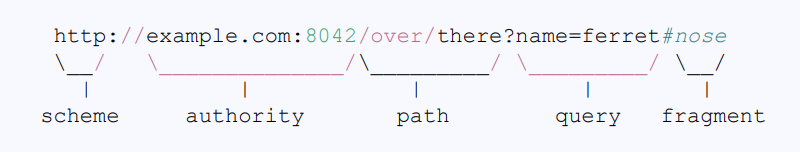
\includegraphics[scale=0.45]{rozdziały/images/AWWW/uri.png}    
\end{center}
\end{example}

\subsection{Express}

\begin{example}
Najprostszy serwer w Node.js
    \begin{js}
import * as http from 'http';
const requestListener = function (req, res) {
  res.writeHead(200);
  res.end('Hello, World!');
}
const server = http.createServer(requestListener);
server.listen(8080)
    \end{js}
\end{example}

Jednak obsłużenie wielu ścieżek jest problematyczne, ale z pomocą przychodzi nam \textbf{Express}.

\subsubsection{Definicja}
\textbf{Express} - minimalistyczny, lekki framework dla Node.js, który ułatwia tworzenie aplikacji sieciowych i API. Oparty na Node.js i zapewniający prostą ale potężną warstwę abstrakcji dla:
    \begin{itemize}
        \item obsługi żądań HTTP,
        \item zarządzania trasami (routingu),
        \item renderowania widoków.
    \end{itemize}

\subsubsection{Prosta aplikacja Express}

\begin{js}
import express from 'express';

let app = express();
app.get('/', (req, res) => {
  res.status(200).send('<!doctype html><title>Strona.</title>')
});
app.listen(8080);
\end{js}

W tak zdefiniowanej aplikacji, serwer otrzymujący żądanie, które nie jest obsługiwane, zwraca odpowiedź ze statusem 404 - Not Found.

\subsubsection{Routing}
\textbf{Routing} to mechanizm, który umożliwia mapowanie żądań HTTP na odpowiednie funkcje obsługujące te żądania. Pozwala to na definiowanie różnych ścieżek (URL) i określanie, jak serwer powinien odpowiedzieć na żądania wysłane do tych ścieżek.

\textbf{Definicja trasy (route) w Express}: używamy metody odpowiadającej dla danego typu żądania HTTP, np. app.get() dla żądań GET, app.post() dla żądań POST itp. Następnie podajemy ścieżkę (URL) jako pierwszy argument, a jako drugi argument podajemy funkcję obsługującą żądanie dla tej ścieżki. Ta funkcja przyjmuje obiekty req (request) i res (response), które reprezentują żądanie klienta i odpowiedź serwera.

\textbf{Dopasowywanie funkcji:} wywoływana jest pierwsza funkcja, której parametr pasuje do URL z żądania. Zwykle piszemy po jednej funkcji dla danej ścieżki, ale można użyć dodatkowego paramteru \textbf{next}, żeby wywołać kolejną pasującą funkcję:

\begin{js}
app.get('/', (req, res, next) => {
    res.status(200).send('<title>Strona.</title>tak.');
    next();
});

app.get('/', (req, res, next) => {
    console.log('Kolejna pasująca funkcja');
}); 
\end{js}

Zaawansowane doposowywanie ścieżek - \textbf{Parametry w ścieżkach}, czyli dynamiczne dopasowywanie ścieżek:
\begin{itemize}
    \item "\textcolor{purple}{:}" pozwala na użycie dynamicznych identyfikatorów w ścieżce. Dla 
    \jsinline{'/users/:id'} w ciele funkcji możemy się odwołać do podanego id poprzez  \jsinline{const userId = req.params.id;}
    Czyli dla żądania \jsinline{"/users/dynamiczneId"} pole \jsinline{userId} będzie równe \jsinline{"dynamiczneId"}.
    
    \item Podobnie można zrobić bardziej wyszukane dopasowanie, przy użyciu wyrażeń regularnych. Przykładowo \jsinline{"/^\/users\/([a-z\d]+)\$/"}, które dopasowuje ścieżkę /users/{username} tylko dla użytkowników o nazwach składających się z małych liter i cyfr.
    W ciele funkcji można się następnie odwołać do takiego id przy użyciu: \jsinline{const username = req.params[0];}
\end{itemize}


\subsubsection{Middleware}
Może się zdarzyć sytuacja, w której chcielibyśmy zalogować informacje o obsłudze każdego z żądań. Można pisać kod w każdej funkcji obsługującej żądanie, ale to niewygodne - z pomocą przychodzi nam Middleware. Definiuje się je za pomocą \jsinline{app.use()}, wtedy middleware aplikowany jest do każdego żądania.

\begin{example}
\begin{js}
app.use((req, res, next) => {
    console.log('Obsługuję ' + req.path);
    next();
});
\end{js}
    
\end{example}

Jednak można też przy użyciu \jsinline{app.get()}. Przykładowo jeśli chcemy dopasować wszystkie żądania, które zawierają  \jsinline{"users"}.

\begin{example}
\begin{js}    
app.get('/users', (req, res, next) => {
  console.log('Middleware dla ścieżki "/users"');
  // Przekazanie żądania do kolejnego middleware lub docelowej funkcji obsługującej
  next();
});
\end{js}

\end{example}

Ponadto można je wykorysytwać do:

\begin{itemize}
    \item analizy ciasteczek,
    \item sprawdzania praw dostępu,
    \item tworzenia sesji,
    \item i wiele innych...
\end{itemize}


\begin{problems}
    \prob Routing w aplikacjach webowych polega między innymi na
    \answers{uruchamianiu różnych funkcji w zależności od adresu URL}{przesyłaniu pakietów przez odpowiednie routery}{kierowaniu zapytań do różnych serwerów bazodanowych (np. w celu rozłożenia obciążenia)}
    %{TAK}{NIE}{NIE?}
\end{problems}

\section{Django}

% TODO
\begin{editorsnote}
    Rozdział nie jest stworzony -- w roku akademickim, w którym powstało repetytorium, Django nie wchodziło w zakres materiału Aplikacji WWW. W archiwalnych egzaminach licencjackich pojawiło się jednak zadanie na jego temat, stąd decyzja o pozostawieniu tej sekcji do ewentualnego jej napisania.
\end{editorsnote}

\begin{problems}
    \prob Django
    \answers{udostępnia swoje usługi za pomocą protokołu HTTP}{jest rozszerzeniem JavaScriptu}{zawiera warstwę odwzorowania relacyjno-obiektowego}
    % {TAK}{NIE}{TAK}
\end{problems}

\begin{solutions}
    % Julia
    \sol Dla danego stylu (nie są stosowane żadne inne style):
    \begin{css}
        div {color: yellow;}
        div p {color: red;}
        div.p {color: green;}
        p#id {color: green;}
        .x#id {color: black;}
    \end{css}
    i fragmentu HTML
    \begin{html}
        <body>
            <div class="x">
                <p id="id"> XXX </p>
                <p> YYY </p>
                ZZZ
            </div>
        </body>
    \end{html}
    \answerss{napis ,,XXX'' ma kolor zielony}{napis ,,YYY'' ma kolor czerwony}{napis ,,ZZZ'' ma kolor żółty}{TAK}{TAK}{TAK}

    Na początek zauważmy, że selektor \cssinline{div.p} nie ma zastosowania w naszym kodzie, ponieważ nie mamy żadnego znacznika \htmlinline{<div>}, który posiadałby klasę o2 nazwie \texttt{p}. Podobnie jest z selektorem \cssinline{.x#id}, ponieważ nie mamy żadnego znacznika z klasą o nazwie \texttt{x} oraz id o nazwie \texttt{id}.

    \begin{enumerate}[\bf A.]
        \item Do napisu ,,XXX'' pasują kolory żółty, czerwony oraz zielony (z selektora \cssinline{p#id}). Zostanie wybrany selektor \cssinline{p#id}, ponieważ ma największą specyficzność (czyli jest ,,najdokładniejszy'').

        \item Do napisu ,,YYY'' pasują kolory żółty i czerwony. Wybrany zostanie kolor czerwony, ponieważ jego selektor ma większą specyficzność.

        \item Do napisu ,,ZZZ'' pasuje tylko kolor żółty, zatem to on zostanie wybrany.
    \end{enumerate}

%  Kasia K
    \sol Dla fragmentu HTML:
    \begin{html}
        <!DOCTYPE html>
        <html>
        <head><title>t</title>
        <style>
            .foo {color: red;}
            #foo {color: blue;}
            #main p {color: green;}
        </style>
        </head>
        <body>
            <div id="main">
                <p id="foo" class="bar">
                    C
                    <span class="foo"> A </span>
                    B
                </p>
            </div>
        </body>
        </html>
    \end{html}
    \answerss
    {litera ,,A'' jest czerwona}
    {litera ,,B'' jest niebieska}
    {litera ,,C'' jest zielona}
    {TAK}{NIE}{TAK}

    Litery ,,B'' i ,,C'' będą zielone, ponieważ są wewnątrz znacznika \htmlinline{<div>}, którego id to \texttt{main}, i w akapicie \htmlinline{<p>}. Zgodnie z zasadami specyficzności selektorów, jest to bardziej dokładne niż bycie tylko w akapicie o id \texttt{foo}. Litera ,,A'' jest bezpośrednio wewnątrz znacznika \htmlinline{<span>} z klasą \texttt{foo}, więc będzie miała czerwony kolor (selektor \cssinline{.foo} dotyczy bezpośrednio tego elementu, więc ma wyższy priorytet niż \cssinline{#main p}, który jest odziedziczony po rodzicu).

    % filip
    \sol Dany jest kod w języku JavaScript:
    \begin{js}
        let tab = [1, 2, 3, 4];
        tab.s = function() { return this.reduce((s, a) => s + a, 0) }
        let t = "";
    \end{js}
    Wartość t będzie równa "1234" (bez cudzysłowu) po wykonaniu fragmentu kodu
    \answerss{\jsinline{for (let i in tab) t = t + tab[i];}}{\jsinline{for (let e in tab) t = t + e;}}{\jsinline{for (let e of tab) t = t + e;}}{NIE}{NIE}{TAK}
    Kod w podpunkcie \textbf{A.} przeiteruje się po każdym kluczu w obiekcie \texttt{tab} i doklei do napisu \texttt{t} wartość pod tym kluczem. Wynikiem nie będzie tu napis \texttt{"1234"}, ponieważ istnieje też klucz \texttt{"s"}. Po tym fragmencie kodu w \texttt{"t"} będzie napis \texttt{"1234function() \{ return this.reduce((s, a) => s + a, 0) \}"}.
    
    Kod w podpunkcie \textbf{B.} z pewnością nie da w wyniku \texttt{"1234"}, ponieważ dokleja do \texttt{t} nazwy kluczy, czyli da w wyniku \texttt{"0123s"}.
    
    Kod z podpunktu \textbf{C.} spowoduje ustawienie \texttt{t} na napis \texttt{"1234"}. Należy pamiętać, że pętla \texttt{for ... of} nie iteruje się po prostu po wartościach kluczy, a wykonuje specjalną iterację zdefiniowaną przez dany obiekt. Dla list pętla ta iteruje się ,,klasycznie'' -- po prostu po elementach listy. Ponieważ atrybut pod kluczem \texttt{"s"} nie jest elementem listy, to nie będzie uwzględniony podczas iteracji.

    % filip
    \sol Domknięcia w języku JavaScript:
    \answerss{pozwalają emulować zmienne prywatne}{służą do realizacji mechanizmu wyjątków}{można zaimplementować w CSS}{TAK}{NIE}{NIE}
    W podpunkcie \textbf{A.} emulację obrazować może przykładowy kod:
    \begin{js}
        var myBankAccount = (function(){
          var balance = 0;
        
          return {
            getBalance: () => balance
          }
        })()
    \end{js}
    Rozgryźmy powyższy kod. Na początek widzimy funkcję, w której deklarowana jest zmienna \texttt{balance}, po czym zwracany jest obiekt, w którym jedynym atrybutem jest funkcja \texttt{getBalance()} zwracająca wartość zmiennej \texttt{balance}. Funkcja ta jest anonimowa i natychmiastowo wywoływana. W wyniku tego, do zmiennej \texttt{myBankAccount} przypisany zostaje wyżej wspomniany obiekt z funkcją zwracającą wartość \texttt{balance} z domknięcia. Ponadto, nie ma żadnego sposobu na dostanie się do tej zmiennej oprócz otrzymania jej wartości poprzez ww. funkcję.
    
    W podpunkcie \textbf{B.} odpowiedzią jest \texttt{NIE}, bo wyjątki są zrealizowane natywnie i bynajmniej nie korzystają z domknięć.
    
    W podpunkcie \textbf{C.} oczywiście odpowiedzią jest \texttt{NIE}, ponieważ domknięć nie ma w CSS.

    % filip
    \sol Dany jest kod w JavaScripcie:
    \begin{js}
        var a = 1;
        function f() {
            console.log(a);
            var a = 2;
            console.log(a);
        }
        f();
        console.log(a);
    \end{js}
    Po jego wykonaniu
    \answerss{w pierwszej linii wyjścia pojawi się wartość \texttt{undefined}}{w drugiej linii wyjścia pojawi się wartość 2}{w trzeciej linii wyjścia pojawi się wartość 2}{TAK}{TAK}{NIE}
    W pierwszej linii wyjścia pojawi się \texttt{undefined}, ponieważ zmienna \texttt{a} została zadeklarowana w ciele funkcji \texttt{f()}, ale zainicjowana dopiero po pierwszym \texttt{console.log(a)}.
    
    W drugiej linii wyjścia pojawi się \texttt{2}, ponieważ zmienna \texttt{a} została już zainicjowana.
    
    W trzeciej linii wyjścia pojawi się \texttt{1}, a nie \texttt{2} -- pomimo że przypisanie wewnątrz funkcji \texttt{f()} zachodziło względem zmiennej o nazwie \texttt{a}, to była to wersja lokalna dla ciała tej funkcji, która jedyne co miała wspólnego z wersją zadeklarowaną globalnie to nazwa. W związku z tym, ponieważ jesteśmy poza ciałem funkcji \texttt{f}, zmienna \texttt{a} nadal ma wartość 1.

    %Tomek
    \sol Routing w aplikacjach webowych polega między innymi na
    \answerss{uruchamianiu różnych funkcji w zależności od adresu URL}{przesyłaniu pakietów przez odpowiednie routery}{kierowaniu zapytań do różnych serwerów bazodanowych (np. w celu rozłożenia obciążenia)}{TAK}{NIE}{NIE}
    
    Z definicji routingu w aplikacjach webowych -- jest to mechanizm, który umożliwia mapowanie żądań HTTP na odpowiednie funkcje obsługujące te żądania. Wynika stąd, że ani podpunkt \textbf{B.}, ani podpunkt \textbf{C.} nie są prawdziwe. Zachodzi jedynie \textbf{A.}

    \sol Django
    \answerss{udostępnia swoje usługi za pomocą protokołu HTTP}{jest rozszerzeniem JavaScriptu}{zawiera warstwę odwzorowania relacyjno-obiektowego}{TAK}{NIE}{TAK}
    
\end{solutions}
